BERTopic è l'unico modello, tra quelli presi in esame, in grado di effettuare una \textbf{topic extraction}, ovvero identificare autonomamente pattern ricorrenti ad un corpus di documenti. Questa caratteristica lo rende particolarmente adatto per il caso di studio, poiché permette di individuare argomenti comuni per grandi volumi di testo, senza alcuna necessità di supervisione umana. \vspace{7pt} \\
A livello implementativo, è stata sviluppata una forma avanzata dell'algoritmo, denominata \textbf{Zero-Shot Topic Modeling}. Mediante questa modalità è possibile elencare le categorie che con maggiore probabilità saranno presenti all'interno dei dati testuali. Tuttavia, questo metodo non si limita solamente a rilevare gli argomenti selezionati, ma possiede le capacità essenziali per generare nuovi topic per tutti quei documenti che non rientrano nell'elenco predefinito. \vspace{7pt} \\
Per applicare Zero-Shot Topic Modeling, sono stati specificati due attributi fondamentali durante la fase di istanziazione del modello, quali:
\begin{itemize}
    \renewcommand{\labelitemi}{-}
    \item \textbf{zeroshot\_topic\_list}. \\
    Lista di topic da assegnare ai documenti. I nomi delle categorie devono essere più descrittivi possibile, poiché l'assegnazione si basa sulla somiglianza per coseno tra gli embedding: maggiore sarà la correlazione con il contenuto testuale, più probabile sarà l'assegnazione.
    \item \textbf{zeroshot\_min\_similarity}. \\
    Soglia minima di similarità da considerare durante l'attribuzione dei topic per ciascun documento, si tratta di un valore reale appartenente all'intervallo chiuso e limitato $\left[0,1\right]$. Minore sarà la soglia, maggiore sarà la probabilità che BERTopic assegni ai documenti la lista predefinita di etichette.
\end{itemize}
Come anticipato dalla descrizione dei parametri, è emersa l'esigenza di convertire le osservazioni del dataset in rappresentazioni numeriche. In questa circostanza, BERTopic offre una discreta libertà decisionale in cui generare gli embedding, secondo due approcci distinti. Nel primo caso, adeguato durante l'analisi, la conversione viene generata in una fase preliminare per poi essere assegnata al modello, riducendo i tempi di esecuzione. Nel secondo caso, la trasformazione avviene internamente all'algoritmo durante l'elaborazione dei documenti; sebbene possa rappresentare una scelta più comoda, può comportare ad un aumento dei tempi di attesa.
\begin{lstlisting}[language=python, caption=Definizione della lista di topic e 
degli embeddings]
from sentence_transformers import SentenceTransformer

# List of predefined topics to use during the topic extraction
list_topics = sum([item for item in topics.values()], [])

# Creating embeddings
docs = list(df_cleaned_preprocessed.Abstract)
embedding_model = SentenceTransformer("all-mpnet-base-v2")

embeddings = embedding_model.encode(docs)
\end{lstlisting}
\begin{lstlisting}[language=python, caption=Creazione e fitting del modello BERTopic]
from bertopic import BERTopic

model = BERTopic(zeroshot_topic_list=list_topics, zeroshot_min_similarity=.6)

_topics, _ = model.fit_transform(docs, embeddings=embeddings)
\end{lstlisting}
Infine, per visualizzare i risultati ottenuti, è stato utilizzata la funzione \textbf{.get\_topic\_info()}, la quale restituisce un dataframe contenente le informazioni principali recuperate durante le attività di topic modeling.
\begin{lstlisting}[language=python, caption=Recupero e visualizzazione del dataset finale generato da BERTopic]
df_bertopic = model.get_topic_info()
display(df_bertopic)
\end{lstlisting}
\begin{figure}[H]
    \centering
    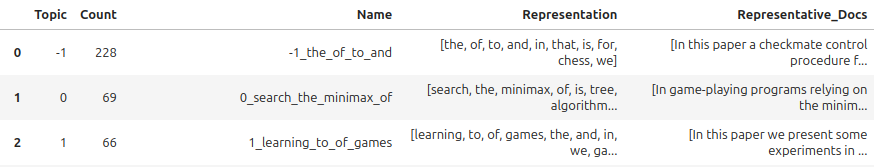
\includegraphics[width=1.0\textwidth]{img/img7.png}
    \caption{Porzione del dataset finale generato da BERTopic}
\end{figure}
Nonostante molteplici esecuzioni, adeguando le categorie descritte nel Paragrafo \ref{4.1}, BERTopic ha dimostrato difficoltà nell'assegnare argomenti predefiniti alla raccolta di documenti. Inoltre, come si evince dalla raffigurazione, alcuni di essi non sono stati nemmeno inclusi all'interno di un qualche insieme creato autonomamente dall'algoritmo. Una motivazione di tale comportamento, seppur marginale, potrebbe consistere nella mancata precisione del modello nel distinguere dati testuali che discutano temi simili o affini. Causa che potrebbe essere imputata all'impiego di una similarità per coseno, che non sempre riesce a catturare sottili differenze semantiche tra tematiche strettamente correlate. Pur di verificare la credibilità dell'ipotesi avanzata, nel Paragrafo \ref{4.4} è stato effettuato un ulteriore esperimento utilizzando documenti che trattassero argomenti differenti. \vspace{7pt} \\
Concludendo, per maggiore chiarezza, è riportata una tabella contenente delle brevi descrizioni delle colonne del dataset ottenuto da BERTopic.
\begin{table}[H]
    \begin{tabularx}{\textwidth}{|c|X|X|}
        \hline
        \small 1. & \small \textbf{Topic} & \small Identificatore numerico del topic \\
        \hline
        \small 2. & \small \textbf{Count} & \small Numero di documenti a cui è stato attribuito il topic \\
        \hline
        \small 3. & \small \textbf{Name} & \small Nome del topic, appartenente all'elenco predefinito oppure generato automaticamente dal modello \\
        \hline
        \small 4. & \small \textbf{Representation} & \small Lista delle parole chiave su cui si formalizza la correlazione tra documenti e topic \\
        \hline
        \small 5. & \small \textbf{Rapresentative Docs} & \small Lista dei documenti considerati rappresentativi per lo specifico topic \\
        \hline
    \end{tabularx}
    \caption{Tabella contenente le features del dataset ottenuto tramite BERTopic}
\end{table}